\frame{
\frametitle{SOM basics}

\begin{columns}

\begin{column}{.6\textwidth}

\begin{itemize}

\item SOM forms a semantic map where similar samples are mapped close together
and dissimilar ones apart. This may be visualized by a U-Matrix (Euclidean
distance between vectors of neighboring cells) of the SOM.

\item Neurons are pointers to the input space. They form a discrete
approximation of the distribution of training samples. More neurons point to
regions with high training sample concentration and fewer where the samples are
scarce.

\end{itemize}

\end{column}

\begin{column}{.4\textwidth}

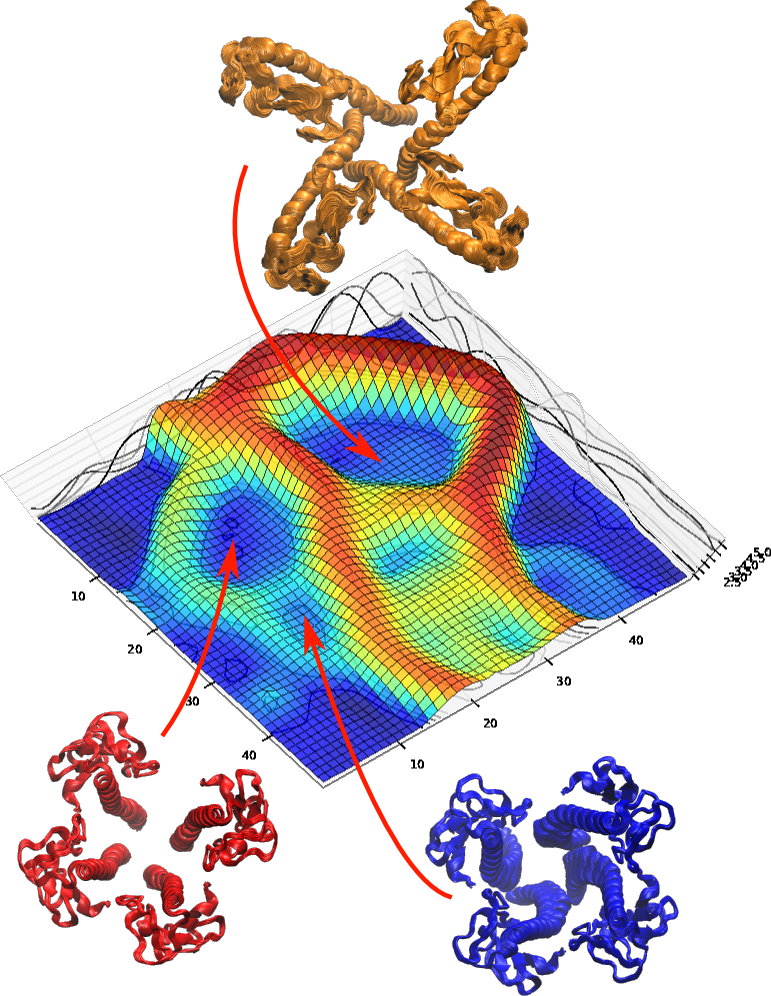
\includegraphics[width=\textwidth]{figures/umatrix3Dinputspace.png}

\small{$$\mbox{U-height}(\nu) = \frac{1}{8}\sum_{\mu \in N(\nu)}d({\nu},{\mu})$$}

\end{column}

\end{columns}
}
